
%(BEGIN_QUESTION)
% Copyright 2006, Tony R. Kuphaldt, released under the Creative Commons Attribution License (v 1.0)
% This means you may do almost anything with this work of mine, so long as you give me proper credit

Identify how to increase the integration time (the number of minutes per repeat) of this pneumatic controller:

$$\includegraphics[width=15.5cm]{i01598x01.eps}$$

Also, determine whether this is a {\it proportional + integral} (PI) controller, or an {\it integral-only} (I) controller, and explain your reasoning.

\vskip 20pt \vbox{\hrule \hbox{\strut \vrule{} {\bf Suggestions for Socratic discussion} \vrule} \hrule}

\begin{itemize}
\item{} How would you modify this mechanism for the opposite direction of action (e.g. direct versus reverse)?
\item{} Explain how this mechanism would respond to an error (PV $-$ SP) if the restrictor valve were placed in-line with the lower-left bellows rather than the upper-left bellows as shown.
\item{} Suppose both the output and reset bellows were replaced with bellows having the same surface area but more volume (i.e. {\it longer} bellows).  What effect(s) would this alteration have on the {\it gain} of the controller, and also the {\it integral time constant} of the controller?
\item{} Suppose both the output and reset bellows were replaced with wider bellows having larger surface areaa as well as more volume.  What effect(s) would this alteration have on the {\it gain} of the controller, and also the {\it integral time constant} of the controller?
\item{} Is it possible to adjust the gain of this controller without affecting its integral time constant, by only changing one aspect of it (e.g. moving a bellows, moving the fulcrum, etc.)?  Explain why or why not.
\item{} Note that this pneumatic controller lacks the {\it bias spring} seen on P-only pneumatic controllers.  Explain why this is.
\item{} Suppose some water vapor in the compressed air supply condensed into liquid water, settling at the bottom of the reset bellows.  What effect(s) might this have on the performance of the controller, if any?  
\end{itemize}

\underbar{file i01598}
%(END_QUESTION)





%(BEGIN_ANSWER)

Close off the valve to increase $\tau_i$ in this PI controller.

%(END_ANSWER)





%(BEGIN_NOTES)

Closing off the valve will result in a decreased air flow rate into or out of the upper bellows for any given amount of error between PV and SP, thus making the output pressure change at a slower rate over time.

\vskip 10pt

We may determine what control modes a controller has by its response to a sudden application (a ``step change'') in error (PV $-$ SP).  The output signal of an integral-only controller will simply begin to ramp when it encounters a sudden error signal.  The output signal of a proportional+integral controller will suddenly ``step'' in response to a sudden error signal, {\it then} ramp at a rate determined by the error signal's magnitude.

Since the output signal of this pneumatic controller immediately ``jumps'' when an error is applied to it, we know it exhibits proportional action as well as integral action.  Thus, it is a PI, or P+I, controller.  It is {\it not} an integral-only, or ``floating response,'' controller.

%INDEX% Control, proportional + integral: pneumatic force-balance controller

%(END_NOTES)


